\documentclass[11pt]{article}
\usepackage{geometry} 
\geometry{a4paper,top=3cm,bottom=3cm,left=2.5cm,right=2.5cm}   
\usepackage{multicol}
\usepackage[english, italian]{babel}
\usepackage{fancyhdr}
\usepackage{lettrine}
\usepackage{musicography}
\geometry{centering}
\usepackage{graphicx}



\pagestyle{fancy}                                 %serve ad inserire la linea sopra e il titolino
\rhead{\textsf{Riprodotto da Hi-Fi News, Agosto 1970}}
\renewcommand{\headrulewidth}{5pt} %grandezza della linea in alto
\renewcommand{\footrulewidth}{1pt}   % grandezza della linea in basso


\begin{document}
\begin{minipage}{0.55\linewidth}
\vspace{0.3cm}
{\large{\textbf{\textsf{Michael Gerson}}}}\\\end{minipage}

\begin{minipage}{0.95\linewidth}
\begin{center}
{\huge{\textbf{\textsf{Surround sound from 2-channel stereo}}}} \\

\end{center}
\end{minipage}
\vspace*{0.3cm}


%=========ARTICOLO========================

\begin{multicols*}{2}
\parskip=0pt

Recentemente c’è stato un grande interesse nella riproduzione sonora quadrifonica (4-canali). Generalmente si ritiene che siano necessari quattro canali per riprodurre il vero “stereo surround”, ma questo articolo descrive un modo per ottenere un vero effetto stereo surround da registrazioni stereo convenzionali a due canali. Per ottenere il suono quadrifonico dalle normali registrazioni stereo, sono necessari due sistemi stereo e può essere sperimentato facilmente da persone che hanno amici con sistemi stereo simili. Non sono richieste particolari abilità elettroniche o pratiche per installare l’apparecchiatura per la riproduzione stereo a quattro altoparlanti e gli appassionati di hi-fi in tutto il paese potrebbero dare un prezioso contributo alla conoscenza della quadrifonia segnalando le proprie esperienze con il tipo di disposizione a quattro altoparlanti descritto di seguito.

Peter Bouwer (nel numero di Aprile) ha descritto un metodo simile per riprodurre lo stereo tramite quattro altoparlanti, ma il metodo descritto in questo articolo differisce dal fatto che è in grado di riprodurre in modo autentico suoni che sembrano provenire tutto intorno l’ascoltatore, invece di produrre semplicemente l’illusione di un ulteriore spazialità.

A prima vista, può sembrare impossibile riprodurre nastri o dischi stereo in modo che i suoni sembrino provenire da tutto intorno all’ascoltatore. Tuttavia, ci sono abbastanza informazioni in eccesso contenute in molti normali segnali stereo che consentono la riproduzione di suoni da dietro l’ascoltatore, nonché da ciascun lato e dalla parte anteriore. L’allestimento sperimentale utilizzato dall’autore compre quattro altoparlanti e due amplificatori stereo, con gli altoparlanti disposti come in Fig.1 I suoni trasmessi ai quattro altoparlanti erano i seguenti: l’altoparlante di sinistra era alimentato con il canale stereo sinistro, l’altoparlante destro veniva alimentato con il canale stereo destro, l’altoparlante anteriore veniva alimentato con la somma dei due canali stereo e l’altoparlante 

\begin{center}
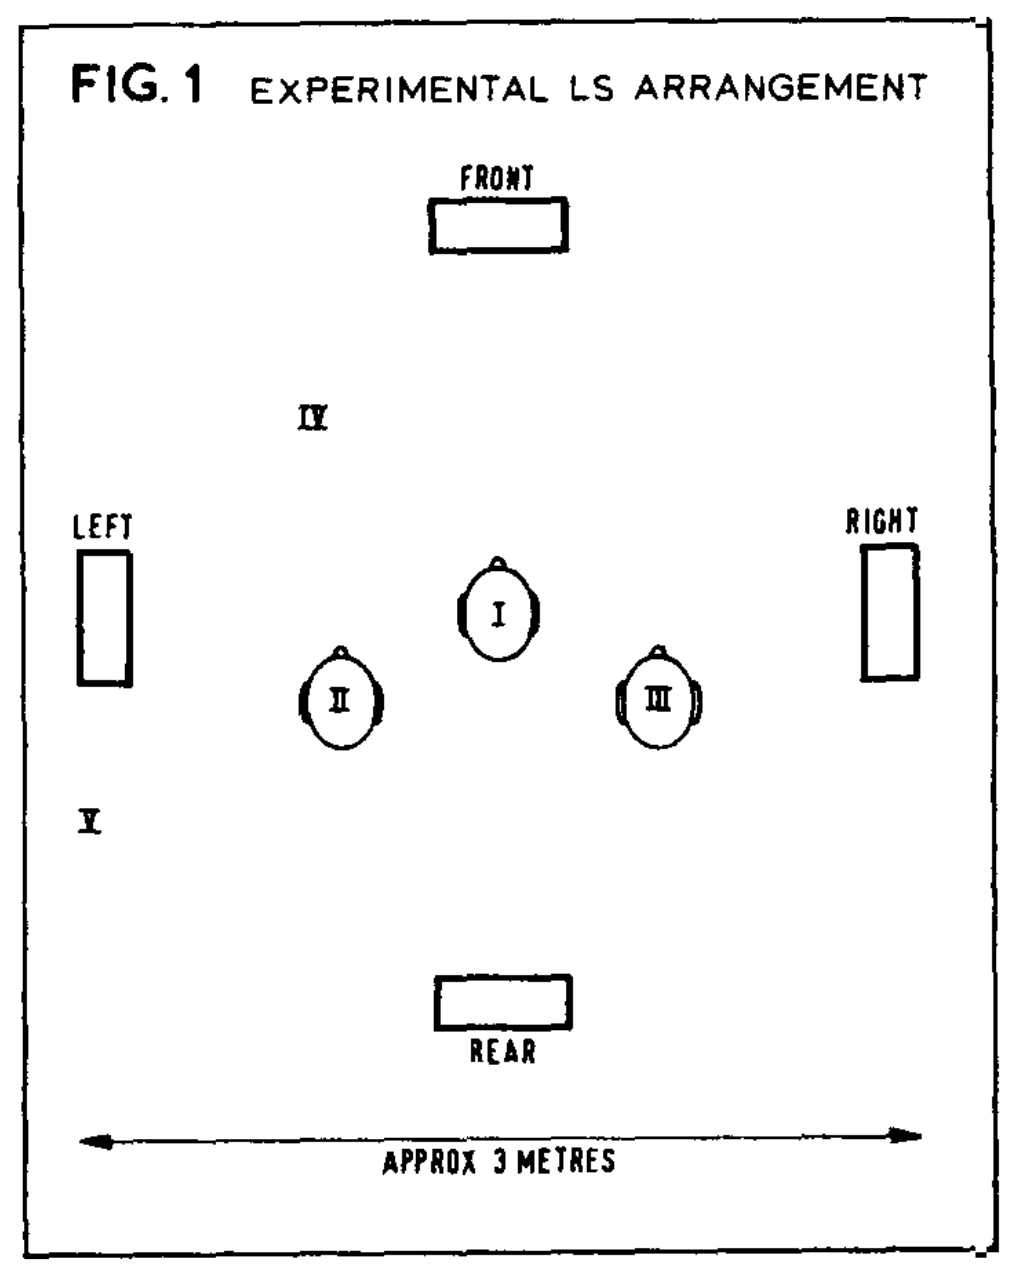
\includegraphics[scale=0.4]{images/fig_01.png}

{\scriptsize \emph{fig.1 }}
\end{center}

 posteriore veniva alimentato con la differenza tra i due canali stereo. L'intenzione è che un suono che viene registrato solo sul canale stereo sinistro verrà riprodotto forte dall'altoparlante di sinistra, e più silenziosamente dagli altoparlanti anteriori e posteriori, e per niente dall'altoparlante di destra; quindi il suono sembrerà provenire dalla sinistra dell'ascoltatore. 


Allo stesso modo, un suono che viene registrato solo sul canale stereo destro sembrerà provenire dalla destra dell'ascoltatore. Un suono che viene registrato allo stesso modo su entrambi i canali stereo verrà riprodotto forte dall'altoparlante anteriore, e più silenziosamente da ciascuno degli altoparlanti laterali e per nulla dall'altoparlante posteriore, e un tale suono sembrerà provenire da davanti all'ascoltatore. Un suono che viene registrato fuori fase sui due canali stereo, ma ugualmente forte su ciascuno, verrà riprodotto forte dall'altoparlante posteriore, meno forte dagli altoparlanti laterali e per nulla dall'altoparlante anteriore; un suono così fuori fase sembrerà provenire da dietro l'ascoltatore. (Si dice che un segnale stereo è fuori fase se il segnale audio sul canale stereo destro ha la polarità opposta al segnale sul canale stereo sinistro.) È quindi possibile riprodurre suoni provenienti da tutto l’ascoltatore. 

Prima di entrare nel metodo dettagliato di cablaggio di una tale configurazione a quattro altoparlanti "somma-e-differenza", vale la pena di descrivere come funziona questo metodo di riproduzione stereo. Chiaramente, le prestazioni del set-up dipenderanno dagli altoparlanti usati, dalla stanza in cui sono collocati, dove sono posizionati gli altoparlanti, dalla natura e dalla fonte della registrazione stereo riprodotta e da dove gli ascoltatori si siedono rispetto agli altoparlanti . Qui posso solo descrivere le esperienze di un set-up ma questo può aiutare come guida per provare questo sistema di riproduzione. 

L'allestimento sperimentale (nella sala comune di Pusey House, Oxford) era come in Fig. 1, e raffigurato con gli altoparlanti collocati in una quadrato la cui diagonale era di poco più di tre metri. Gli altoparlanti utilizzati erano Quad Electrostatics, alimentati da quattro amplificatori valvolari Quad II tramite due unità di controllo stereo Quad 22. Un'unità di controllo controllava gli altoparlanti anteriori e posteriori, l'altra controllava gli altoparlanti laterali. È stato quindi possibile controllare in modo indipendente il bilanciamento e il volume da sinistra a destra, nonché il bilanciamento e il volume da anteriore a posteriore. La fonte del programma era un registratore a nastro Revox F36HS.

La maggior parte delle registrazioni riprodotte su questo set erano master-tape stereo di concerti dal vivo registrati dalla Oxford University Tape Recording Society. Questi master-tape sono stati tutti registrati utilizzando una coppia di microfoni a nastro coincidenti, uno montato immediatamente sopra l’altro, entrambi Reslo VRT o STC 4038. Tutti gli ascoltatori di questo esperimento avevano familiarità con questi nastri riprodotti tramite Quad Electrostatics in stereo normale e conoscevano il suono dal vivo dei vari artisti. Per questo motivo, è stato possibile giudicare quanto fosse realistica la riproduzione dei quattro altoparlanti, senza essere fuorviata da difetti sconosciuti o inganno nelle registrazioni.

Una volta regolati correttamente i livelli relativi dei quattro altoparlanti, tutti gli ascoltatori sono rimasti colpiti dalla qualità realistica e ampia della riproduzione. L'acustica e l'atmosfera degli edifici in cui erano stati registrati i nastri sono stati accuratamente catturati, ma sono stati notati una serie di effetti collaterali indesiderati. Gli ascoltatori seduti al centro dei quattro altoparlanti (posizione I nella Figura 1) hanno scoperto che l'immagine stereo si muoveva rapidamente se si muoveva la testa. Inoltre, su alcuni nastri, alcuni ascoltatori (non tutti) hanno scoperto che alcuni strumenti e artisti sembravano (erroneamente) suonare proprio dietro la testa dell'ascoltatore. Tuttavia, sulla maggior parte dei nastri questo effetto non è stato notato. Un ascoltatore ha osservato che su un nastro aveva la sensazione che c'erano quattro orchestre che suonavano contemporaneamente.

Questo tipo di reazione da parte degli ascoltatori posti nel mezzo dei quattro diffusori era stata prevista. Ciò che non era stato previsto era quanto funzionasse la riproduzione a quattro diffusori di un nastro stereo per gli ascoltatori che non si trovavano al centro. Si è scoperto che è importante che ogni ascoltatore non abbia altri ascoltatori nel percorso del suono da nessuno dei quattro altoparlanti. Posizionando ascoltatori nelle posizioni I, II e III nella Figura 1, è stato possibile per tre ascoltatori ascoltare tutti e quattro gli altoparlanti contemporaneamente. Con sorpresa di tutti, è stato scoperto che gli ascoltatori nelle posizioni II e III hanno ottenuto un suono molto buono, con l'orchestra o il coro che sembra provenire sicuramente di fronte all'ascoltatore. In alcune registrazioni, il suono ottenuto nelle posizioni II e III era effettivamente preferito al suono nella posizione I.

Gli ascoltatori nelle posizioni II e III di Fig. 1 hanno scoperto che l'atmosfera e l'acustica delle sale da concerto in cui sono state effettuate le registrazioni sono state riprodotte con grande realismo e presenza. Una difficoltà psicologica era che era impossibile convincersi che questo suono spazioso, pieno di profondità, proveniva dagli altoparlanti piuttosto vicini, con il risultato che l'immagine tendeva a sembrare innaturale a meno che uno non ignorasse gli altoparlanti o chiudesse gli occhi.

È stato riscontrato che l'altoparlante posteriore ha contribuito pochissimo, e spegnerlo non influiva molto sulla posizione stereo degli strumenti: tuttavia, si notò una perdita di "profondità" quando l'altoparlante posteriore non funzionava. I lettori che possiedono solo un amplificatore mono e un solo altoparlante oltre al loro sistema stereo potrebbero provare a riprodurre lo stereo tramite tre altoparlanti omettendo il canale posteriore. La riproduzione è ancora abbastanza spaziosa e un simile set di tre altoparlanti ha una netta somiglianza con il set di "bi-amplificazione" di Peter Bouwer.

Un effetto sorprendente della riproduzione a quattro altoparlanti è stato il volume puro che poteva essere riprodotto. A causa del fatto che i master-tape dal vivo contengono una buona quantità di alti che non sono stati limitati o rimossi dall'elaborazione tecnica, molte di queste registrazioni tendono a sovraccaricare le configurazioni Quad II/electrostatic nella normale riproduzione stereo a livelli molto inferiori a quelli reali. Si è scoperto che la riproduzione a quattro altoparlanti produceva livelli soggettivi molto più alti prima che iniziasse la distorsione. Nonostante il volume dei climax musicali sembrasse molto alto (come accadeva dal vivo), non vi era alcun senso di tensione o disagio, ma solo un brivido della straordinaria qualità ‘elettrica’ della musica, che lo scrittore ha sperimentato in precedenza solo in concerti dal vivo.

In altre parole, la riproduzione a quattro canali tende ad aumentare il volume apparente di passaggi fortissimo in un modo che riproduce l'enorme potenza e l'effetto della musica dal vivo. I passaggi più silenziosi, tuttavia, hanno mantenuto la loro silenziosità e la riproduzione a quattro altoparlanti sembra preservare la dinamica meglio del normale stereo. Le diverse qualità acustiche delle varie posizioni di registrazione sono state immediatamente evidenti attraverso quattro altoparlanti. Un difetto di questo sistema di riproduzione a quattro altoparlanti era che gli ascoltatori nel mezzo sentivano troppa acustica, sebbene gli ascoltatori nelle posizioni II e III della Fig. 1 trovassero l'acustica abbastanza realistica.

Molti dei nastri dal vivo includevano suoni non musicali come applausi, il coro che camminava sul palco, il pubblico che chiacchierava mentre se ne andava, conversazioni vicino ai microfoni e vari rumori e sussurri associati alle prove. Tali suoni sono stati riprodotti in modo impressionante, con applausi, passi, chiacchericcio, ecc., provenienti da tutto intorno. Particolarmente impressionanti sono state le registrazioni del coro che camminava sul palco oltre i microfoni, in cui i passi degli artisti passavano da dietro l'ascoltatore, alla sua destra, e quindi di fronte a lui. Questi effetti sono stati osservati dagli ascoltatori nelle posizioni I, II e III di Fig. 1. Non sembra esserci alcun dubbio che la tecnica di riproduzione a quattro altoparlanti "somma e differenza" per lo stereo produce un suono a tutto tondo.

Si è riscontrato che la riproduzione a quattro altoparlanti produce un'immagine stereo molto più ampia rispetto allo stereo convenzionale e che la separazione tra strumenti era molto marcata. È stato possibile distinguere tra cantanti in una parte del coro, o violini all'interno dell'orchestra, molto più facilmente rispetto allo stereo a due altoparlanti.

Tuttavia, è stato riscontrato che anche piccole quantità di distorsione offuscavano gravemente l'immagine stereo. In effetti, è stata un'osservazione generale che piccoli difetti di qualità tecnica erano molto più evidenti con la riproduzione a quattro altoparlanti rispetto allo stereo normale. Piccole quantità di distorsione, che sono quasi impercettibili nello stereo normale, sono chiaramente udibili come "intasamento" e "sfocatura" con riproduzione a quattro altoparlanti, e anche i nastri master da 38 cm / sec, registrati a livelli ragionevoli, quando leggermente distorti, se riprodotti attraverso quattro altoparlanti. Il risultato fu che la definizione stereo tendeva a sfocare durante i climax della musica.

Una perdita generale di realismo è stata anche rilevata a causa della risposta in frequenza delle registrazioni. Secondo la maggior parte degli standard, i diffusori Quad e i microfoni STC 4038 sono considerati davvero eccellenti, ma è noto che gli STC cadono giù gradualmente sopra i 7kHz e gli altoparlanti Quad sopra i 12kHz. Il risultato è che i nastri stereo riprodotti tramite quattro altoparlanti suonavano piuttosto opachi rispetto al suono live; questa opacità è meno discutibile nello stereo normale, poiché lo stereo normale suona comunque piuttosto opaco e senza vita rispetto alla realtà.

Gli ascoltatori nella posizione IV della Fig. 1 hanno scoperto che la maggior parte del suono sembrava provenire da dietro, il che è stato molto sconcertante. D'altra parte, gli ascoltatori al di fuori del quadrato degli altoparlanti, come nella posizione V della Fig. 1, hanno scoperto di aver udito un suono stereo spazioso e piacevole, sebbene questo suono non circondasse più completamente l’ascoltatore.

Oltre ai master-tape di musica dal vivo, è stata tentata la riproduzione di trasmissioni stereo della BBC. Mentre lo stereo della BBC si basa spesso su una coppia di microfoni coincidenti, i microfoni aggiuntivi vengono spesso utilizzati per "evidenziare" i solisti o per aggiungere riverbero. In generale, le recenti trasmissioni della BBC hanno trasmesso relativamente poco del suono acustico e hanno suonato estremamente secche sugli altoparlanti Quad. Lo stereo della BBC, riprodotto tramite quattro altoparlanti, è risultato più ricco e spazioso rispetto a quando riprodotto su due altoparlanti. Tuttavia, l'acustica secca con la riproduzione a quattro altoparlanti non ha dato praticamente nessuna sensazione di essere effettivamente nella sala da concerto, e si è ritenuto che lo stereo della BBC non sfruttasse appieno i vantaggi della riproduzione a quattro altoparlanti. La definizione dello stereo della BBC su quattro altoparlanti è risultata piuttosto peggiore di quella dei master-tape.

Come esperimento finale, alcune registrazioni stereo dei Beatles sono state riprodotte tramite quattro altoparlanti, ma i risultati sono stati piuttosto deludenti per due motivi. In primo luogo, lo stereo proveniva da dischi di grammofono e le sottili distorsioni inevitabili con il disco tendevano ad essere molto più evidenti, come spiegato in precedenza. In secondo luogo, il recente stereo dei Beatles è registrato con una tecnica "pan-pot", in cui ogni strumento o cantante si trova registrato su una traccia mono separata e inserito nell'immagine stereo alimentando le tracce con volumi diversi nei due canali stereo. Se riprodotto tramite quattro altoparlanti, ciò produceva un effetto stereo piuttosto scadente e non era sempre facile dire da dove provenisse un suono. Quelli con un arrangiamento musicale molto semplice sembravano funzionare meglio.

Riassumendo, la tecnica di somma e differenza a quattro altoparlanti per la riproduzione di registrazioni stereo può aumentare enormemente il realismo di registrazioni con microfoni coincidenti del tipo "figura otto", ma ha meno successo con le tecniche di registrazione stereo più artificiali. Il fatto che vengano usati solo due canali per fornire il suono a quattro altoparlanti significa inevitabilmente che la riproduzione non è perfetta in ogni modo, ma è comunque sorprendentemente buona. Chiaramente, adeguate tecniche di registrazione a tre o quattro canali dovrebbero essere in grado di fare ancora meglio.

Ora possiamo tornare agli aspetti tecnici quando ci sono chiaramente problemi nel trovare un modo per collegare i quattro altoparlanti. I segnali inviati agli altoparlanti destro e sinistro possono essere ottenuti collegando la sorgente (nastro stereo, disco o radio) in un amplificatore stereo come di consueto. Il problema principale è derivare i segnali per gli altoparlanti anteriori e posteriori, che devono essere alimentati da un secondo amplificatore a due canali.

Ricordiamo che il segnale da inviare all'altoparlante anteriore è la somma dei due canali stereo. Nel nostro setup sperimentale, questo segnale è stato ottenuto collegando le uscite del canale destro e sinistro del registratore in un attenuatore 220K che sono stati collegati, tramite un adattatore a Y (cioè un dispositivo che consente a due cavi di essere collegati a una presa), nell’ingresso sinistro di una seconda unità stereo Quad; l'amplificatore corrispondente alimentava l'altoparlante anteriore (vedi Fig. 2). L'altoparlante posteriore deve essere alimentato con la “differenza" dei segnali tra il canale destro e sinistro. Si può ricavare la differenza tra i due canali combinando l'uscita del registratore a nastro sinistro con un segnale di polarità inversa a destra tramite un attenuatore e un adattatore a Y alimentato all'ingresso destro del secondo amplificatore stereo. Sfortunatamente, è necessario un circuito di inversione di fase, con un guadagno di meno uno, per invertire la polarità del segnale di destra.

Mentre quelli con esperienza nell'elettronica possono costruire un invertitore di fase abbastanza facilmente, quelli con amplificatori a valvole Quad non devono farlo. Nell'unità di controllo Quad 22, il percorso tra l'ingresso di alto livello e l’uscita 1 ha un guadagno di -1; in altre parole, per un segnale di alto livello immesso nell’ingresso, i preamplificatori Quad contengono un invertitore di fase incorporato. Pertanto, se il primo amplificatore (che alimenta i diffusori laterali) è un Quad, allora si ottiene il segnale di differenza da collegare al secondo amplificatore combinando l'uscita sinistra del registratore con l'uscita destra del primo Quad tramite due attenuatori e un adattatore a Y. Questo segnale di differenza viene inviato all'ingresso destro del secondo amplificatore, che viene connesso all'altoparlante posteriore (vedere la Figura 2). Vorrei ringraziare Peter Craven per aver suggerito di utilizzare il Quad come un invertitore di fase in questo modo - una tecnica che non funzionerà con il Quad 33, anche se altri progetti potrebbero essere adatti.


\begin{center}
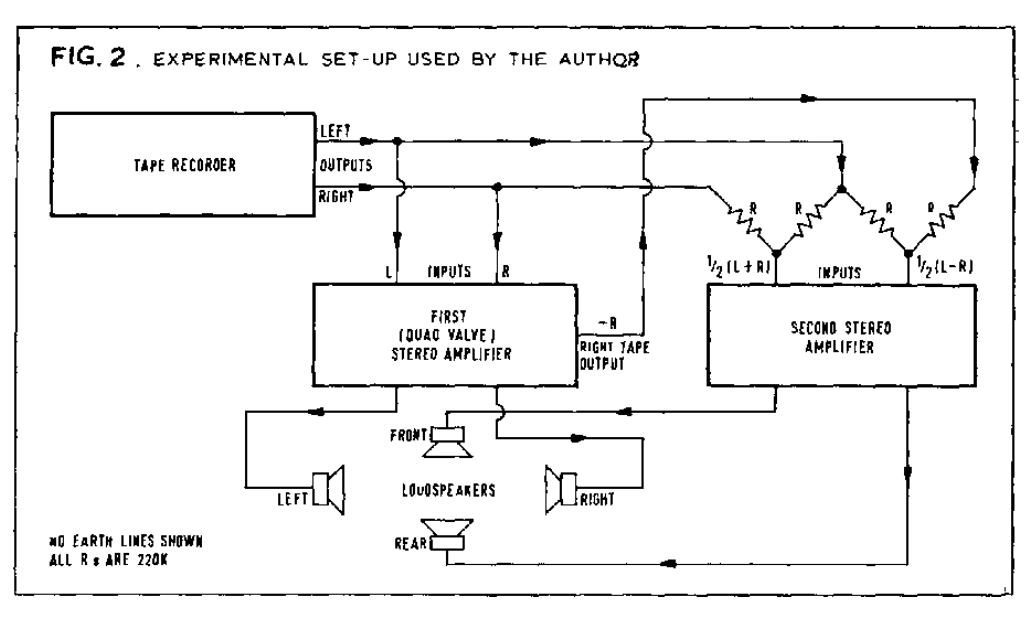
\includegraphics[scale = 0.43]{images/fig_02.png}


{\scriptsize \emph{fig.2 }}
\end{center}

La disposizione presentata sopra ha lo svantaggio di poter essere utilizzata solo con sorgenti di alto livello non bilanciate come nastri o radio. Coloro che sono in grado di costruire invertitore di fase (o che dispongono di trasformatori che possono essere utilizzati come invertitori di fase) possono anche utilizzare sorgenti di basso livello ed equalizzate (come il disco) derivando i segnali per il secondo amplificatore dalle uscite del primo amplificatore, che non deve quindi essere un Quad. Il vantaggio dei metodi di cui sopra per derivare i segnali degli altoparlanti anteriori e posteriori è che i livelli inviati a tutti e quattro gli altoparlanti possono essere regolati indipendentemente l'uno dall'altro. Inoltre, se gli altoparlanti anteriori e posteriori differiscono dagli altoparlanti laterali, è possibile regolare il "tono" degli altoparlanti anteriori e posteriori in modo che corrisponda a quello degli altoparlanti laterali.

Se il lettore non ha un amplificatore con inversione di fase incorporato o se manca il tempo o le conoscenze per costruirne uno, esiste un altro metodo per ottenere i segnali di "somma e differenza", che ha anche il vantaggio di può essere utilizzato con ingressi equalizzati di basso livello come il disco. Collegare i segnali sinistro e destro da disco, nastro o radio al primo amplificatore stereo come di consueto; questo amplificatore alimenta gli altoparlanti laterali. Prendi i segnali sinistro e destro dall'uscita del primo amplificatore e immetti il segnale di uscita sinistro nell'ingresso di alto livello sinistro del secondo amplificatore (vedi Fig. 3) e connetti il segnale di uscita sinistro e destro del primo amplificatore tramite un attenuatore (ad es. 220 K) e un adattatore a Y all'ingresso di alto livello destro del secondo amplificatore. L'altoparlante anteriore viene quindi pilotato dall'uscita dell'altoparlante destro del secondo amplificatore, poiché deve riprodurre la somma dei canali stereo originali. Le due messe a terra del secondo amplificatore stereo sono unite e l'altoparlante posteriore è collegato tra il “live terminal” dell'uscita dell'altoparlante sinistro e il “live terminal” del dell’altoparlante destro. (Ciò potrebbe causare danni a volumi alti con alcuni amplificatori a transistor economici, ma dovrebbe essere sicuro con buone apparecchiature a volumi normali).

Un suono mono centrale (ad es. Un disco mono riprodotto con l'apparecchiatura commutata su stereo) dovrebbe quindi essere riprodotto sul sistema e il controllo del bilanciamento del secondo amplificatore dovrebbe essere regolato con cura per ridurre al minimo l'uscita dell'altoparlante posteriore. Fatto ciò, l'altoparlante posteriore dovrebbe riprodurre la differenza tra i due canali stereo e, in seguito, il controllo del bilanciamento del secondo amplificatore non dovrebbe essere toccato.



\begin{center}
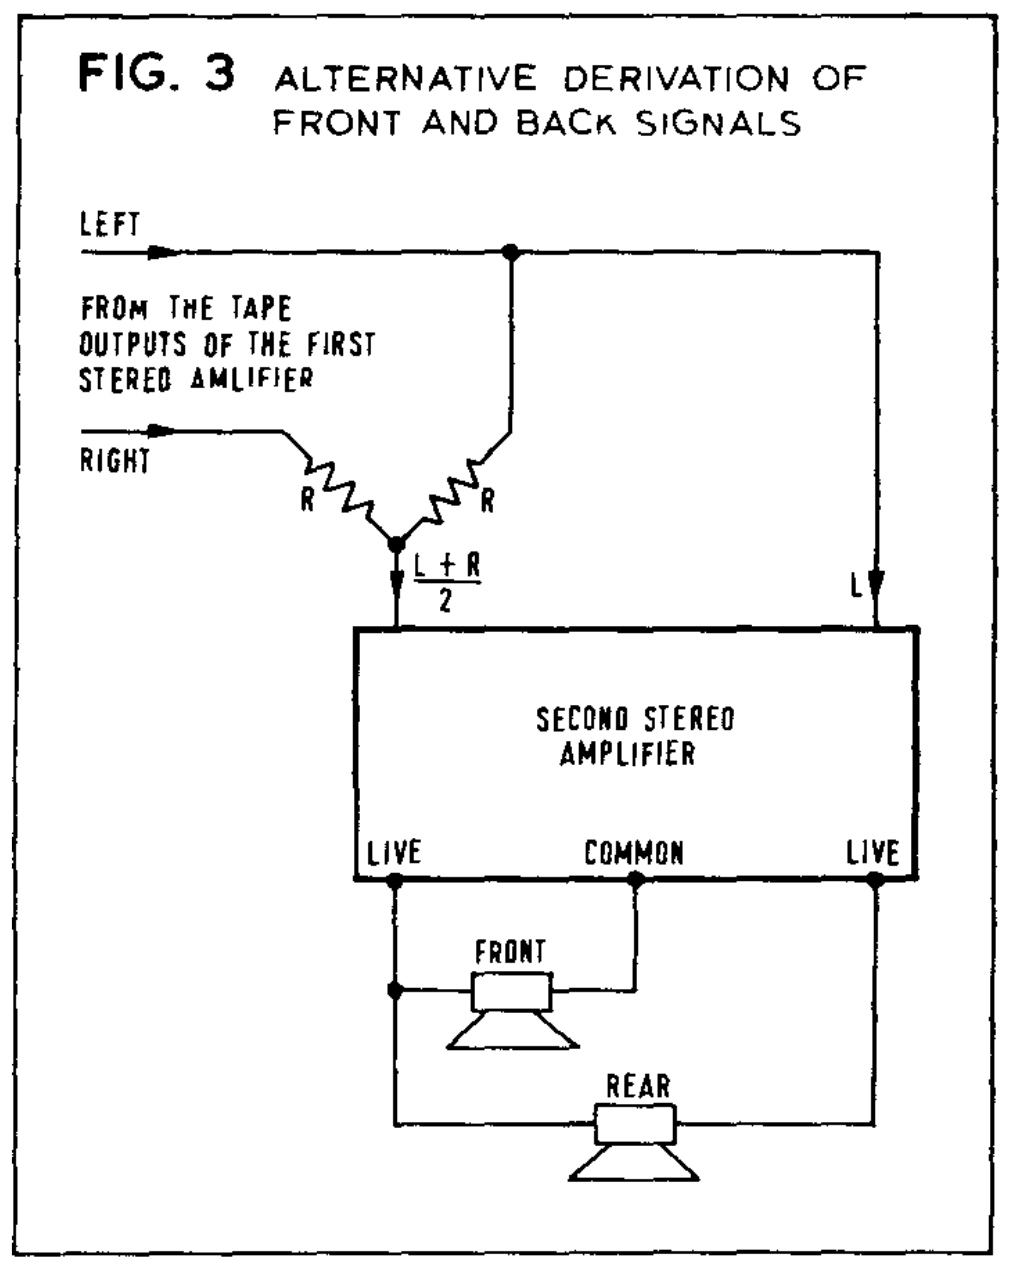
\includegraphics[scale=0.4]{images/fig_03.png}


{\scriptsize \emph{fig.3}}
\end{center}

Uno svantaggio di questo metodo per ottenere i segnali di somma e differenza è che non è possibile controllare separatamente i livelli dell'altoparlante anteriore e dell'altoparlante posteriore. Un secondo svantaggio è che il metodo di collegamento degli altoparlanti anteriori e posteriori pone ulteriori requisiti sull'amplificatore. Questo svantaggio può essere minimizzato utilizzando altoparlanti da 15 ohm anziché 8 ohm.

Qualunque sia il metodo utilizzato, è necessario prestare attenzione a eliminare gradualmente i tre altoparlanti anteriori. Non è buono fare affidamento solo sul modo in cui i cavi sono collegati ai terminali dell'amplificatore e dei diffusori, come se l'altoparlante anteriore avesse un segnale derivato dalle uscite del nastro del primo amplificatore, è possibile che le uscite del nastro siano state alterate in fase. La fase dell'altoparlante anteriore dovrebbe essere raggiunta, ad esempio, posizionando temporaneamente l'altoparlante anteriore accanto, per esempio, all'altoparlante sinistro, e determinando quale fase per l'altoparlante anteriore produce la maggior parte dei bassi su suoni mono bassi. Non esiste una fase "corretta" per l'altoparlante posteriore e la sua fase dovrebbe essere regolata per ciò che l'ascoltatore ritiene sia la migliore riproduzione a quattro altoparlanti.
Ma la fase dell'altoparlante posteriore non fa molta differenza.

I segnali inviati al secondo amplificatore possono provenire dall'uscita del preamplificatore del primo amplificatore, quindi le regolazioni di volume e tono sul primo amplificatore influenzeranno tutti e quattro gli altoparlanti. Tuttavia, in tal caso il controllo del bilanciamento del primo preamplificatore deve essere lasciato al centro, altrimenti influirà sulla miscelazione del suono trasmesso agli altoparlanti anteriori e posteriori. Per ridurre al minimo la perdita degli acuti, è consigliabile posizionare tutti gli attenuatori il più vicino possibile al secondo amplificatore. È possibile posizionare quattro altoparlanti per la riproduzione di "somma e differenza" in stanze piuttosto piccole posizionandole come in Fig 4; tuttavia, molte persone potrebbero pensare che guardare nell'angolo della stanza rovini piuttosto il godimento musicale. 

\begin{center}
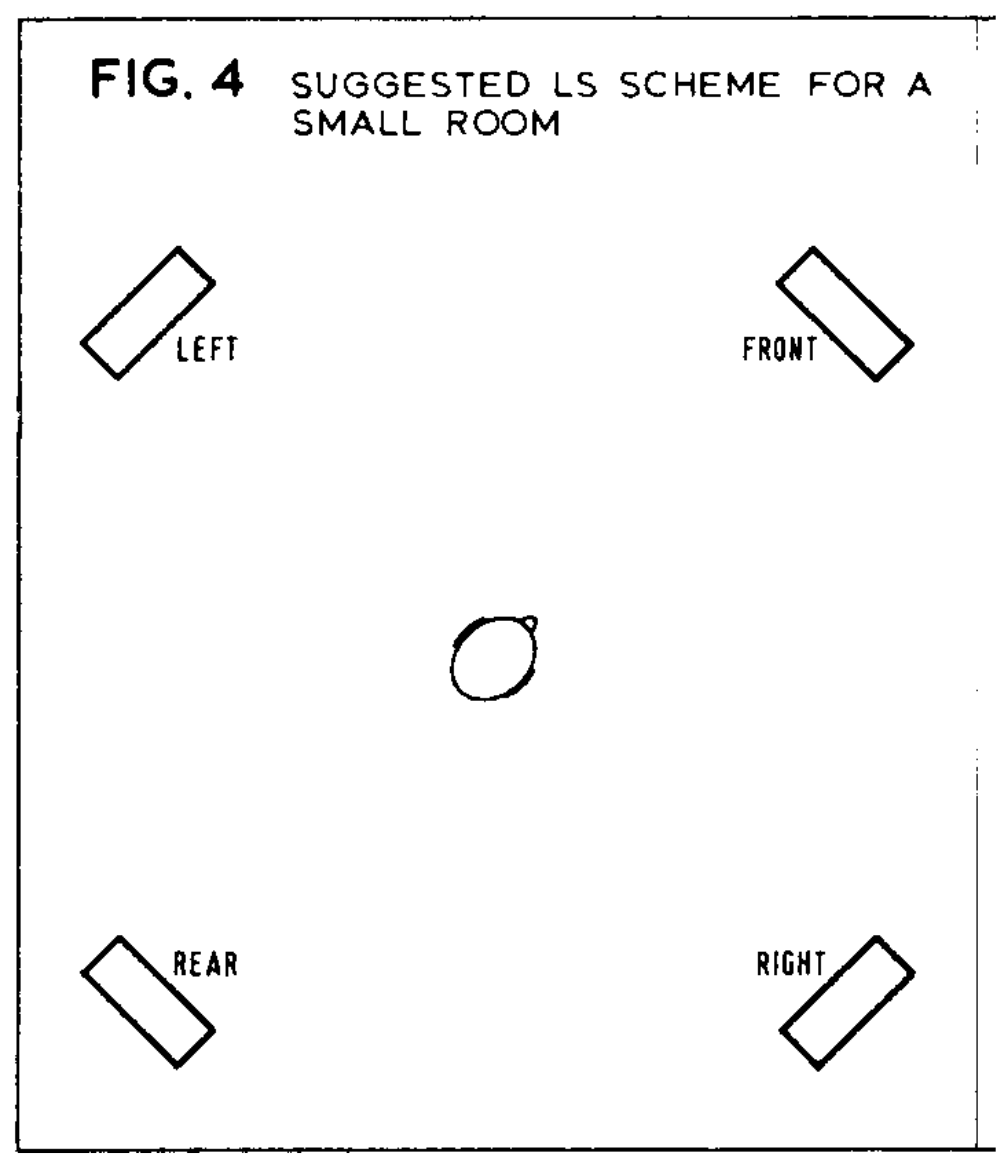
\includegraphics[scale=0.4]{images/fig_04.png}

{\scriptsize \emph{fig.4}}
\end{center}


Una comprensione più completa di come la riproduzione di quattro altoparlanti "somma e differenza" di opere stereo può essere ottenuta considerando la riproduzione dei suoni raccolti da una coppia di microfoni stereo Blumlein. Sarà quindi evidente che, nonostante i buoni risultati, ci sono alcune imperfezioni intrinseche in questo metodo di riproduzione stereo. Il metodo più semplice per registrare l'audio stereo è la tecnica Blumlein, in cui vengono utilizzati due microfoni quasi coincidenti con caratteristiche direzionali "figura di otto". Il microfono del canale sinistro è puntato 45o verso sinistra, e il microfono del canale destro è puntato 45o verso destra, come illustrato nella Figura 5.

\begin{center}
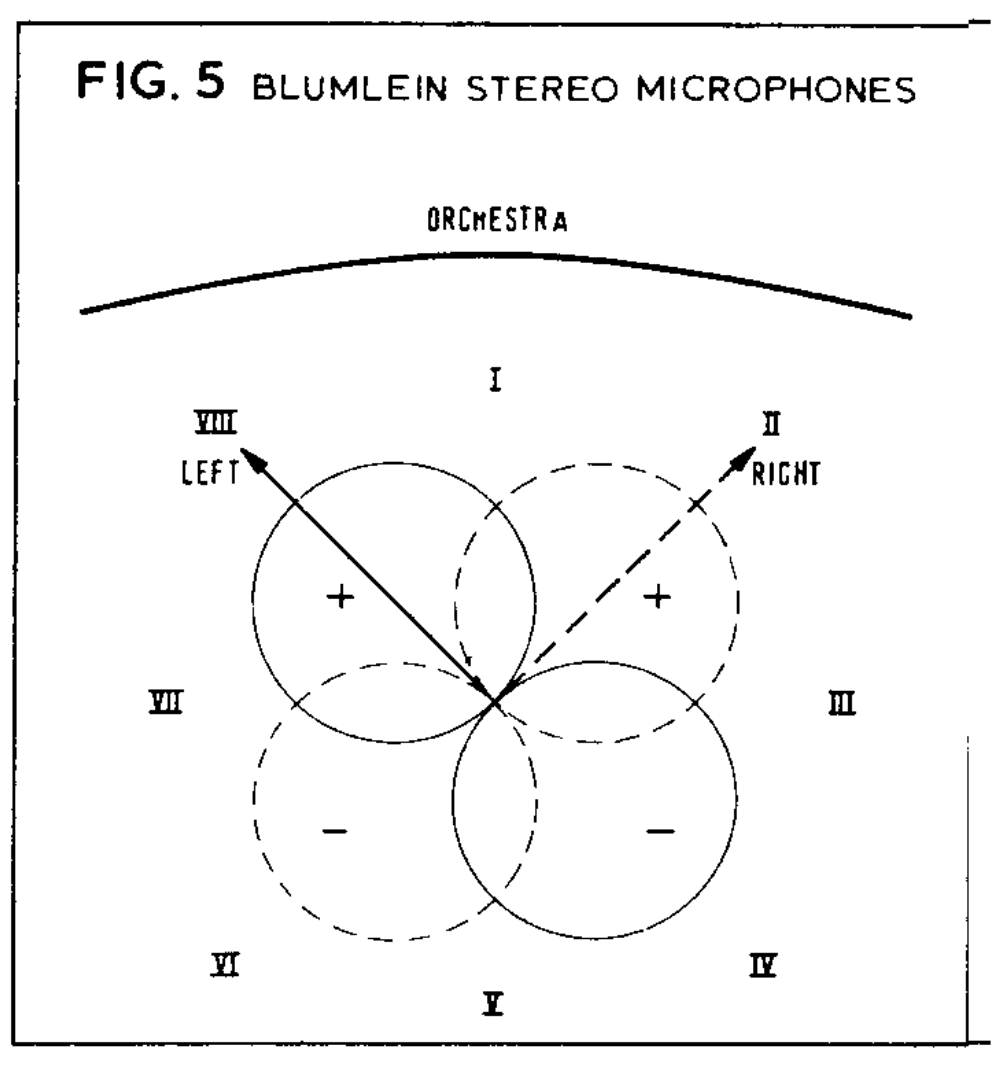
\includegraphics[scale=0.43]{images/fig_05.png}

{\scriptsize \emph{fig.4}}
\end{center}

Un suono dal vivo nella posizione I di Fig 5 (dritto davanti ai microfoni) verrà riprodotto dalla parte anteriore di un ascoltatore che ascolta tramite la somma e differenza quattro
impostazione degli altoparlanti. Un suono dalla posizione II di Fig 5 verrà raccolto solo sul canale destro, quindi verrà riprodotto a destra dell'ascoltatore. Un suono dalla posizione III di Fig 5 verrà raccolto come segnale stereo fuori fase, quindi verrà riprodotto da dietro l'ascoltatore. Allo stesso modo, i suoni delle posizioni IV, V, VI, VII e VIII di Fig 5 saranno riprodotti, rispettivamente, a sinistra, davanti, a destra, dietro e a sinistra dell’ascoltatore.

Il risultato è che un altoparlante o un musicista che cammina una volta attorno ai microfoni stereo verrà riprodotto come se stesse girando due volte attorno ai quattro altoparlanti. La riproduzione stereo a quattro altoparlanti non riproduce la direzione originale del suono e fa sì che la larghezza riprodotta delle immagini stereo sia doppia rispetto alla larghezza live originale. Una conseguenza matematica indiretta di ciò è che non tutti e quattro gli altoparlanti possono essere correttamente messi in fase, ed è per questo che l'altoparlante posteriore non ha una fase corretta, indebolendo inevitabilmente la solidità e l'impatto delle immagini sul retro dell’ascoltatore.

Se per effettuare una registrazione stereo vengono utilizzati microfoni cardioidi distanziati o coincidenti, nessun suono verrà registrato fuori fase e tali registrazioni verranno riprodotte su quattro altoparlanti senza alcun suono proveniente da dietro l'ascoltatore. Mancheranno molto della "profondità" e della spaziosità delle registrazioni Blumlein riprodotte tramite quattro altoparlanti e probabilmente suoneranno altrettanto bene se l'altoparlante posteriore è scollegato. Tuttavia, molte registrazioni della BBC sono fatte con "crossed cottage-loaves 
" (gergo della BBC per microfoni ipercardioidi coincidenti incrociati) e queste registrazioni dovrebbero riprodurre una buona dose di atmosfera da dietro l’ascoltatore.

Un altro, più ovvio, difetto della riproduzione a quattro altoparlanti "somma e differenza" è la disposizione dei posti estremamente scomoda, che non è adatta per l'accogliente godimento domestico della musica. Domesticamente si vorrebbe usare una disposizione degli altoparlanti come in Fig 6, con altoparlanti posteriori sinistro, anteriore sinistro, anteriore destro e posteriore destro. Chiaramente, con questa disposizione degli altoparlanti, le proporzioni del segnale stereo sinistro L e del segnale stereo destro R che devono essere inviate ai quattro altoparlanti è diversa dalle proporzioni nel layout "somma e differenza”.

Etichettando i segnali inviati ai quattro altoparlanti A, B, C e D come in Fig 6, i segnali sono derivati da L e R come indicato lì. Questi coefficienti sono scelti in modo che i suoni stereo vengano riprodotti dai quattro altoparlanti dalla stessa direzione apparente, rispetto all'ascoltatore, come nel layout di somma e differenza. Sebbene l'autore non abbia provato il sistema di riproduzione di Fig 6, molto probabilmente soffrirà di difetti simili a quelli del layout "somma e differenza". In particolare, gli altoparlanti posteriori sono sfasati l'uno rispetto all'altro.
Il successo generale, sulle registrazioni musicali e naturali, della riproduzione stereo a quattro altoparlanti indica che le registrazioni quadrifoniche correttamente registrate dovrebbero essere qualcosa di cui non vediamo l'ora. Nel frattempo, molte grazie a Peter Craven e Stephen Thornton per i loro commenti costruttivi e il loro aiuto, e a Philip Allen per la sua infinita pazienza.





\end{multicols*}

\end{document}